
This chapter evaluates the implemented prototype against the requirements
defined in Section~\ref{sec:requirements_analysis}. The evaluation
examines the correctness of natural-language intent processing,
action-specific relationship verification, and the maintenance of
verification knowledge. It also considers the traceability of
verification decisions, verification latency, and the controlled
handover of approved operations to smart-wallet execution.

The experimental evaluation separates intent processing from graph
verification to assess both stages independently and prevent
interpretation errors from being concealed by an apparently correct
final decision. It also distinguishes graph approval from transaction
preparation and blockchain execution. An approval indicates that the
requested operation is consistent with the admitted verification
knowledge within the supported prototype scope, but does not
guarantee successful execution. The chapter is divided into two parts. The experimental evaluation
presents the evaluation goals, methodology, results, and discussion,
including threats to validity. It examines the individual processing
stages and the complete verification pipeline, together with
knowledge-maintenance scenarios and supplementary execution-control
tests. The requirements evaluation then assesses the fulfilment of
requirements R1 to R6 using the experimental findings and compares the
prototype with the approach groups discussed in the state of the art
analysis.


% ### 5.1 Evaluation Goals ###

\section{Evaluation Goals}
\label{sec:evaluation_goals}

The main goal of the evaluation is to assess whether the implemented
prototype can correctly interpret natural-language DeFi requests and
verify the execution relationships required by the requested operations.
The evaluation focuses on Uniswap V3 swaps and Aave V3 lending operations
on Ethereum Sepolia. It examines the individual processing stages and
their interaction, with particular attention to preventing the approval
of operations that are inconsistent with the admitted verification
knowledge.

The evaluation addresses six research questions derived from the
requirements defined in Section~\ref{sec:requirements_analysis}:

\begin{enumerate}
    \item[\textbf{Q1:}] How accurately does the language model extract
    the requested action, protocol, assets, amount, network, and
    additional constraints, and how reliably do normalization and
    deterministic validation handle incomplete, ambiguous, or
    unsupported requests?

    \item[\textbf{Q2:}] Can graph-based verification correctly distinguish
    valid execution relationships from invalid combinations of known
    entities? How does the verifier respond when the available
    knowledge is incomplete, outdated, or unavailable?

    \item[\textbf{Q3:}] To what extent does the complete verification
    pipeline preserve the intended operation and its constraints
    while producing the appropriate verification decision?

    \item[\textbf{Q4:}] What proportion of eligible graph-verification
    requests is completed within the two-second threshold defined
    in R6, and how does verification latency vary across the
    evaluated requests?

    \item[\textbf{Q5:}] To what extent do the verification results
    provide sufficient evidence to identify the relevant execution
    relationships, validation conditions, and reasons for
    non-approval?

    \item[\textbf{Q6:}] To what extent do the implemented execution
    controls prevent unapproved, modified, expired, or previously
    used operations from proceeding toward transaction submission?
\end{enumerate}

The first three questions address intent processing, relationship
verification, and the interaction between these stages. Evaluating
intent processing and graph verification independently allows errors
introduced during interpretation or validation to be distinguished
from errors in the verification mechanism. The evaluation also
examines whether explicit relationship checks can identify invalid
execution paths that would remain undetected when only the existence
of individual entities is considered. Knowledge-maintenance
experiments complement these tests by examining how changes in
the available evidence affect verification decisions. The remaining questions concern the operational properties of the
prototype. Verification latency is assessed against the quantitative
requirement R6, while traceability is evaluated through the evidence
returned with each decision. The controlled execution handover is
examined separately to assess the implemented restrictions on
approved operations. This supplementary evaluation does not aim
to establish successful blockchain execution or the complete
security of the connected wallet.

The experimental findings provide the basis for assessing the
fulfilment of requirements R1 to R6 and comparing the prototype
with the approach groups examined in the state-of-the-art analysis.
The evaluation considers both the contribution of action-specific
relationship verification and the limitations arising from
natural-language interpretation, verification knowledge, and
execution controls.


% ## 5.2 Methodology ##

\section{Evaluation Methodology}
\label{sec:evaluation_methodology}

The evaluation examines intent processing and graph verification separately
before assessing their combined behaviour. Two natural-language request studies
are considered: an exploratory study with 400 prompts conducted on 19 and
20 October 2026, and a balanced follow-up with 600 prompts conducted from
22 to 24 October 2026. The studies use different datasets and are analysed
separately. Controlled experiments on graph relationships, knowledge
maintenance, traceability, and wallet handover provide additional evidence
about properties that cannot be established through prompt testing alone.

\subsection{Test Material and Reference Data}
\label{sec:evaluation_test_material}

The balanced dataset comprises 300 scenarios, each expressed in two formulations
intended to preserve the same operation and constraints.\footnote{The two
formulations belong to the same underlying scenario. They are used to examine
wording sensitivity and must not be treated as independent test cases.}
The resulting 600 prompts are distributed equally across six categories, as
shown in Table~\ref{tab:evaluation_dataset}. The supported operations are
single-hop Uniswap V3 ERC-20 swaps and Aave V3 supply, withdraw, borrow, and
repay on Ethereum Sepolia, with chain ID~11155111
\cite{implUniswapSingleSwap,implAavePool}.\footnote{The evaluated Uniswap
operation uses one pool for an exact-input swap. Requests requiring an
intermediate token or a multi-hop route are outside the prototype scope.}

\begin{table}[htbp]
    \centering
    \small
    \caption{Composition of the balanced request dataset.}
    \label{tab:evaluation_dataset}
    \begin{tabular}{p{0.63\linewidth}rr}
        \hline
        \textbf{Request category} & \textbf{Scenarios} & \textbf{Prompts} \\
        \hline
        Supported Uniswap V3 swaps & 50 & 100 \\
        Supported Aave V3 operations & 50 & 100 \\
        Known entities with invalid relationships & 50 & 100 \\
        Unknown or unsupported entities and operations & 50 & 100 \\
        Incomplete or ambiguous requests & 50 & 100 \\
        Invalid parameters or unsupported conditions & 50 & 100 \\
        \hline
        \textbf{Total} & \textbf{300} & \textbf{600} \\
        \hline
    \end{tabular}
\end{table}

The first two categories represent operations expected to be supported by the
admitted graph snapshot. The remaining categories examine different grounds
for non-approval, including invalid relationships, unsupported scope, and
missing information. Equal category sizes facilitate comparison but do not
reflect the frequency of these requests in actual DeFi use. 


The evaluation requests were constructed synthetically rather than
sampled directly from an existing transaction dataset. The six
categories in Table~\ref{tab:evaluation_dataset} provided the basis
for scenario construction. Supported requests were developed using
the implemented operations and the admitted Sepolia graph snapshot.
The remaining categories represented invalid execution relationships,
unsupported scope, incomplete or ambiguous instructions, and
invalid parameters or unsupported conditions.

For each category, 50 scenarios were prepared with assistant support,
using protocol documentation, the implemented prototype, the saved
graph snapshot, and observations from development. Each scenario
specified the intended operation or failure condition, the relevant
constraints, and the expected verification outcome. Where applicable,
the corresponding structured intent and required graph relationships
were also recorded. Two natural-language formulations were then
prepared for each scenario, with the intention of preserving the same
operation and constraints. This produced 300 scenarios and 600 prompts.

Examples from INTENT-TX-18K informed the earlier exploratory work,
but the balanced dataset consists of newly constructed scenarios
rather than unchanged records from that dataset.\footnote{raw dataset
\url{https://github.com/duanyiyao/intent-tx-18k/blob/main/dataset/eg_uniswap_samples.json}.}
Omitted networks use the configured Sepolia context, whereas
explicitly conflicting networks are unsupported.

Both datasets were executed using saved assistant-drafted references. Their
item-level independent human review was not documented. The 600-prompt
execution copy was locked before the run, but this does not make its labels
independently validated ground truth. The follow-up was informed by earlier
failures; screening also identified overlapping graph inputs and closely
related scenarios. Accordingly, the evaluation reports agreement with draft
references rather than validated population accuracy. Reference revisions,
if made after examining the results, must be documented separately without
replacing the original labels.

\subsection{Experimental Procedure}
\label{sec:evaluation_procedure}

The extraction component used the Groq-hosted model
\texttt{openai/gpt-oss-20b}. For the balanced run, temperature was set to zero,
reasoning effort to low, and the maximum completion length to 512 tokens.
One logical pass was completed, with a seeded order that interleaved request
categories and randomized formulation order within each pair. Interrupted
runs resumed from saved checkpoints. Previously recorded responses and
provider errors were retained rather than replaced by successful reruns.

\paragraph{Experiment A: Intent generation and validation.}
Each prompt was processed through language-model extraction, normalization,
and deterministic validation. The recorded raw response, structured intent,
constraint handling, validation disposition, and errors were compared with
the draft reference. Field mismatches were distinguished from cases in which
correctly extracted information was handled incorrectly by validation.
Clarification, unsupported conditions, and service failures were recorded as
separate outcomes.

\paragraph{Experiment B: Independent graph verification.}
Reference intents eligible for graph verification were submitted directly to
the Neo4j verifier, regardless of whether the language model processed their
corresponding prompts correctly. Requests lacking the fields necessary for a
graph decision were excluded from this experiment, with their eligibility
recorded. Predefined parameterized Cypher queries checked the action-specific
relationships against the admitted snapshot \cite{implNeo4jCypher}. Decisions
and selected execution evidence were compared with snapshot-derived reference
values. Counts of eligible calls and distinct graph inputs were maintained
separately because multiple prompts can require identical graph checks.

\paragraph{Experiment C: Complete verification pipeline.}
The recorded output from Experiment A was passed through the remaining
validation and, where eligible, graph-verification stages without manual
correction. Experiments A and C therefore shared the same model generation
for each prompt. Final decisions were compared with the original request's
draft reference, and the earliest identifiable stage of disagreement was
recorded. A graph decision that is correct for an incorrectly reduced intent
was not considered evidence of faithful interpretation of the original
request. The earlier 400-prompt study followed a separate exploratory procedure, with
primary formulations processed before alternatives and a provider-quota
interruption. The balanced follow-up used a different ordering and category
distribution. Its results are not pooled with the exploratory observations or
interpreted as a controlled before-and-after comparison.

\subsection{Controlled Verification and Execution Tests}
\label{sec:evaluation_controlled_experiments}

\paragraph{Experiment D: Relationship mutations.}
Twelve valid fixtures were tested in an isolated Neo4j environment, including
four Uniswap paths and eight Aave action and asset combinations. Each fixture
was evaluated unchanged and after five separate deletions of a required
relationship: action to function, contract to function, deployment to
contract, deployment to resource, and resource to asset. Entities remained
present, and the graph was restored between modifications. This produced
12 controls and 60 mutation cases. The full verifier was compared with an
entity-existence baseline that omitted connected relationship checks but
retained the relevant entity and network restrictions.\footnote{This baseline
isolates the value of checking connected execution paths; it is not a
comparison between Neo4j and an equally expressive relational implementation.}
The mutation cases share the same underlying fixtures and are not treated as
independent security observations.

\paragraph{Experiment E: Knowledge maintenance.}
For each protocol, six controlled conditions were examined: fresh knowledge,
stale knowledge, incomplete coverage, deactivation of an accepted
relationship, failed source acquisition, and database unavailability. The
12 scenarios were repeated three times. The recorded knowledge state,
freshness and coverage information, and verifier outcome were compared with
predefined expectations. Injected failures were distinguished from actual
source or database outages, and an operational failure was not interpreted as
a semantic rejection. A separate traceability audit examined whether verification results contained
an explicit decision, an identifiable rule or reason, the relevant entity or
relationship, and expected and observed values where applicable. Wallet
handover was assessed through existing controlled policy, capability, and
preparation tests, including expired or reused approvals and modified
parameters. These tests address the implemented ERC-4337-based execution
handover \cite{implERC4337}, but simulated wallet outcomes do not demonstrate
successful on-chain execution.\footnote{Graph approval establishes the
relationship checks for the interpreted intent. It does not by itself
establish wallet authorization, sufficient balances or collateral, or
transaction success.} The controlled experiments were conducted separately
from the 600-prompt language study.

A subsequent, separate evaluation examined restricted
smart-wallet authorization using a local EVM environment.
The test environment deployed the actual Kernel 0.3.1 and
ERC-4337 EntryPoint 0.7 contracts together with a custom
permission validator. Authorized operations and deliberately
modified transaction batches were submitted through the
contract-level validation and execution path. The tests
examined contract and function restrictions, parameter
binding, account and network context, permission validity,
and single-use authorization. The local experiments did not
include installation or transaction submission on public
Ethereum Sepolia.

\subsection{Measurements and Analysis}
\label{sec:evaluation_measurements}

Exact final-status agreement is the proportion of attempted prompts whose
observed final disposition matches the draft reference, including operational
errors in the denominator. Joint reference agreement additionally requires
validation-status agreement and matching specified intent fields and
missing-field sets for references expecting approval or clarification. For
other dispositions, the joint measure tests disposition agreement only; it
is not an exhaustive measure of semantic correctness. A secondary binary analysis treats \texttt{APPROVED} as the positive class
and all other normal decisions as non-approval. Precision, recall,
specificity, false-positive rate, false-negative rate, F1 score, and binary
accuracy are calculated from true positives, false positives, false
negatives, and true negatives. These measures use only prompts yielding a
normal decision. Provider and operational errors remain in the attempted
prompt count and are reported separately through decision coverage.\footnote{
An unavailable provider or database does not establish that the requested
operation is unsupported. Such failures must remain distinguishable from
normal verification decisions.} Binary agreement is less strict than exact
status agreement because different non-approval dispositions are combined.

For the paired analysis, observed decisions and draft-reference matches are
compared between the two formulations of each scenario. The designated primary
formulation is also reported separately. Since prompts share scenarios,
templates, and graph inputs, the analysis remains descriptive. Conventional
methods for binomial sample planning and confidence intervals assume an
appropriate sampling model \cite{evalNISTSampleSize,evalNISTConfidence,evalWilson1927}.
Such assumptions were not established here, so no inferential test or
confidence interval treating all 600 prompts as independent trials is used. Verification latency is measured from entry of a complete structured intent
into the graph-verification stage until its result becomes available. The
measurement includes Cypher queries and database processing but excludes
language-model generation, wallet preparation, and blockchain execution.
Requirement R6 specifies that at least 95\% of eligible verification decisions
must be returned within two seconds. The observed proportion is calculated as

\begin{equation}
    P_{\mathrm{R6}} =
    \frac{N_{\leq 2000\,\mathrm{ms}}}{N_{\mathrm{eligible}}}
    \times 100\%.
    \label{eq:evaluation_r6}
\end{equation}

The denominator includes all eligible graph-verification calls started,
including failures and timeouts. First calls and slow observations are
retained. Median, 95th percentile, maximum latency, and the proportion within
the threshold are reported both for all calls and for first occurrences of
distinct graph inputs.

\subsection{Reproducibility and Error Review}
\label{sec:evaluation_reproducibility}

The saved evidence includes dataset and reference versions, scenario identifiers,
model settings, application and graph snapshots, request order, checkpoints,
provider attempts, observed outcomes, timings, and errors. Aggregate
measurements are checked against case-level records; secret credentials and
signing material are excluded. Disagreements are examined using preserved
extraction and validation records, with observed behaviour separated from
retrospective explanations of its cause. Results are presented in
Section~\ref{sec:experimental_results}; their implications and threats to
validity are considered in the subsequent sections.


% 5.3 experimental results

\section{Experimental Results}
\label{sec:experimental_results}

% Restrained palette for thesis figures; defined locally in this section.
% TikZ/PGFPlots loads xcolor. No external chart images are required.
\definecolor{evalBlue}{HTML}{829FB4}
\definecolor{evalTeal}{HTML}{8DACA3}
\definecolor{evalSlate}{HTML}{9EAAB4}
\definecolor{evalRose}{HTML}{CAA5A0}
\definecolor{evalGrid}{HTML}{E8EDF0}
\definecolor{evalInk}{HTML}{2C3A45}
\pgfplotsset{
  evaluationAxis/.style={
    grid style={draw=evalGrid},
    axis line style={draw=evalSlate},
    tick style={draw=evalSlate},
    label style={color=evalInk},
    tick label style={color=evalInk}
  }
}

This section presents the results of the balanced 600-prompt
evaluation, followed by independent graph-verification and
controlled experiments. All agreement values refer to
assistant-drafted references without documented item-level
human review. The experiments did not establish successful
blockchain execution.

\subsection{Natural-Language Request Evaluation}
\label{sec:results_balanced}

% The exploratory study, conducted on 19 and 20 October 2026, contained
% 400 prompts from 200 scenario families. The final disposition matched the
% draft reference for 344 prompts (86.00\%), and 336 (84.00\%) satisfied the
% recorded joint-reference criterion. Three requests ended in provider errors.
% These findings are reported separately because the subsequent dataset had
% a different category distribution and construction procedure.

The balanced evaluation was conducted from 22 to 24 October 2026.
It comprised 300 scenarios, each expressed in two formulations,
resulting in 600 prompts distributed equally across six categories.
Of these attempts, 596 produced a normal decision and four ended
in provider quota errors. Exact final-status agreement with the
draft references was obtained for 534 prompts (89.00\%), while
529 prompts (88.17\%) satisfied the more restrictive joint-reference
criterion.

The joint measure additionally checks specified fields and missing-field sets
for requests expected to be approved or clarified. For other reference
outcomes, it tests the dispositions only and therefore does not establish
complete semantic correctness.

\begin{table}[H]
    \centering\small
    \caption{Principal outcomes of the balanced request evaluation.}
    \label{tab:results_balanced_summary}
    \begin{tabular}{p{0.70\linewidth}r}
    \hline
    \textbf{Measurement} & \textbf{Observed result} \\
    \hline
    Attempted prompts & 600 \\
    Completed decisions & 596 (99.33\%) \\
    Provider quota errors & 4 (0.67\%) \\
    Exact final-status matches & 534 (89.00\%) \\
    Joint draft-reference matches & 529 (88.17\%) \\
    \hline
    \end{tabular}
\end{table}

Figure~\ref{fig:results_category} shows the different outcomes across
request categories. Each category contains 100
prompts, including any operational errors. The joint measure uses the
restricted reference definition described in Section~\ref{sec:evaluation_measurements}. Supported Aave operations and invalid relationships
had high agreement with draft references; incomplete requests had the
lowest agreement.


\begin{figure}[htbp]
\centering
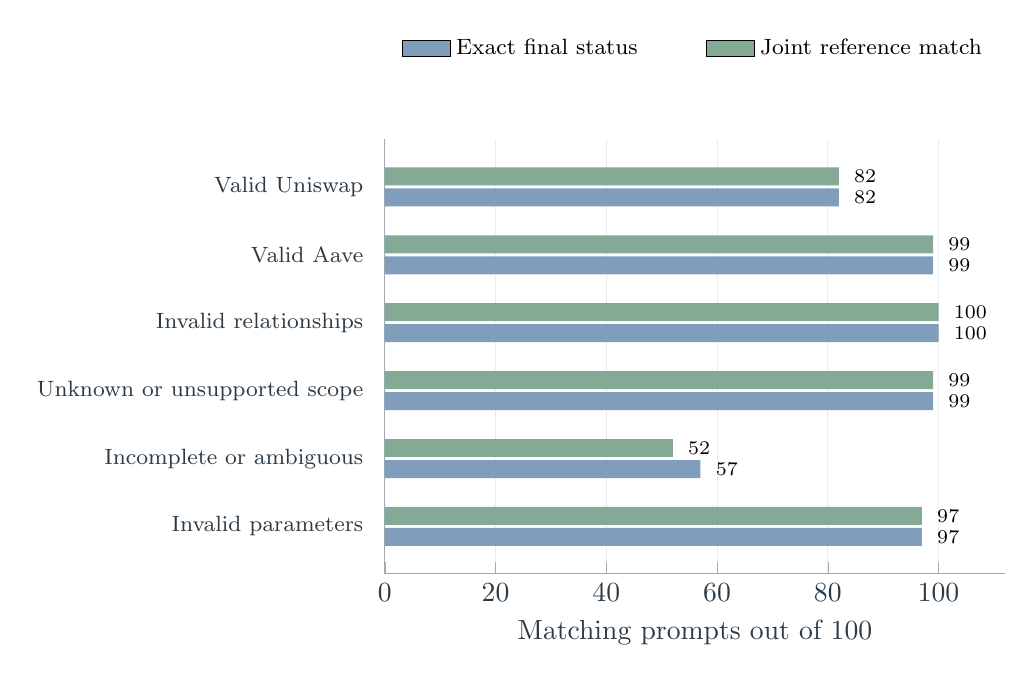
\begin{tikzpicture}
\definecolor{evalBlueSoft}{HTML}{809DBB}
\definecolor{evalGreenSoft}{HTML}{84AA96}
\begin{axis}[
    evaluationAxis,
    xbar,
    width=0.78\linewidth,
    height=7.1cm,
    xmin=0,
    xmax=112,
    xtick={0,20,40,60,80,100},
    xlabel={Matching prompts out of 100},
    xmajorgrids,
    grid style={evalGrid},
    symbolic y coords={
        Invalid parameters,
        Incomplete or ambiguous,
        Unknown or unsupported scope,
        Invalid relationships,
        Valid Aave,
        Valid Uniswap
    },
    ytick={
        Invalid parameters,
        Incomplete or ambiguous,
        Unknown or unsupported scope,
        Invalid relationships,
        Valid Aave,
        Valid Uniswap
    },
    yticklabel style={
        font=\footnotesize,
        text=evalInk
    },
    axis x line*=bottom,
    axis y line*=left,
    ytick style={draw=none},
    enlarge y limits=0.14,
    enlarge x limits=false,
    bar width=6.5pt,
    nodes near coords,
    point meta=x,
    every node near coord/.append style={
        font=\scriptsize,
        anchor=west,
        xshift=2pt
    },
    clip=false,
    legend style={
        at={(0.5,1.16)},
        anchor=south,
        legend columns=2,
        draw=none,
        font=\footnotesize,
        /tikz/every even column/.append style={
            column sep=0.8cm
        }
    }
]
% Exact final-status agreement
\addplot[
    fill=evalBlueSoft,
    draw=none,
    bar shift=-3.8pt,
    forget plot
] coordinates {
    (97,Invalid parameters)
    (57,Incomplete or ambiguous)
    (99,Unknown or unsupported scope)
    (100,Invalid relationships)
    (99,Valid Aave)
    (82,Valid Uniswap)
};
% Joint reference agreement
\addplot[
    fill=evalGreenSoft,
    draw=none,
    bar shift=3.8pt,
    forget plot
] coordinates {
    (97,Invalid parameters)
    (52,Incomplete or ambiguous)
    (99,Unknown or unsupported scope)
    (100,Invalid relationships)
    (99,Valid Aave)
    (82,Valid Uniswap)
};
% Legend with single rectangular symbols
\addlegendimage{area legend,fill=evalBlueSoft,draw=none}
\addlegendentry{Exact final status}
\addlegendimage{area legend,fill=evalGreenSoft,draw=none}
\addlegendentry{Joint reference match}
\end{axis}
\end{tikzpicture}
\caption{Agreement with the draft reference by request
category. Exact final-status agreement considers only
the final disposition, whereas joint reference agreement
also considers selected structured-intent fields.}
\label{fig:results_category}
\end{figure}


The complete outcome matrix in Figure~\ref{fig:results_full_matrix} retains
the distinctions between rejection, unsupported scope, clarification and
operational errors. Rows show draft references and columns the observed outcomes. Quota failures
are retained in the error column and are not counted as correct rejections. Among 100 requests expected to require clarification,
57 received that result, 38 were marked unsupported, four were rejected
and one ended in an error. For the binary assessment, \texttt{APPROVED} is the positive class; all other normal decisions are grouped as non-approval. There were
181 true positives (TP), 396 true negatives (TN), one false positive (FP)
and 18 false negatives (FN). The four quota errors remain outside the
596-decision matrix but are included in the 600-attempt totals.


\begin{figure}[H]
\centering
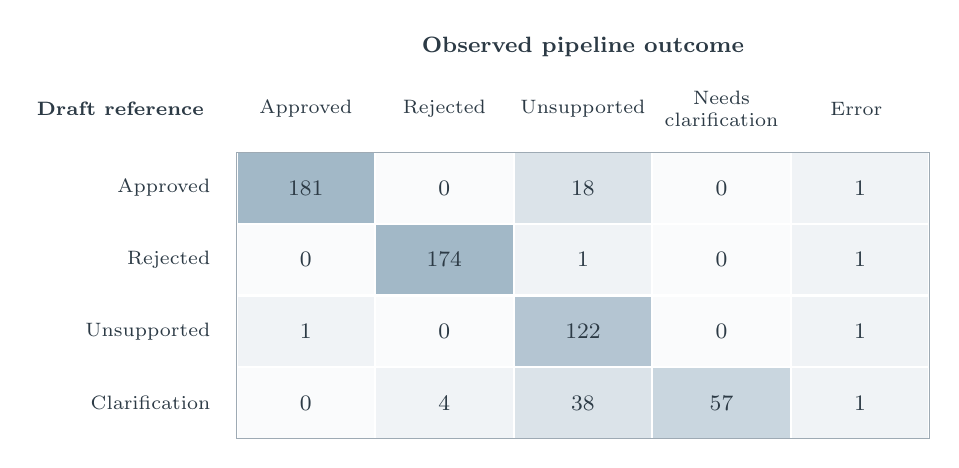
\begin{tikzpicture}[font=\footnotesize, text=evalInk]

    \def\cw{1.76}
    \def\ch{0.91}

    % Column heading
    \node[
        font=\footnotesize\bfseries,
        text=evalInk
    ] at ({2.5*\cw},1.34)
      {Observed pipeline outcome};

    % Row heading
    \node[
        anchor=east,
        font=\scriptsize\bfseries,
        text=evalInk
    ] at (-0.29,0.55)
      {Draft reference};

    % Column labels
    \foreach \x/\lab in {
        0/{Approved},
        1/{Rejected},
        2/{Unsupported},
        3/{\shortstack[c]{Needs\\clarification}},
        4/{Error}
    } {
        \node[
            font=\scriptsize,
            align=center,
            inner sep=1pt
        ] at ({(\x+0.5)*\cw},0.55) {\lab};
    }

    % Row labels
    \foreach \y/\lab in {
        0/{Approved},
        1/{Rejected},
        2/{Unsupported},
        3/{Clarification}
    } {
        \node[
            anchor=east,
            font=\scriptsize,
            inner sep=1pt
        ] at (-0.29,{-(\y+0.5)*\ch}) {\lab};
    }

    % Confusion matrix values
    \foreach \row/\a/\b/\c/\d/\e in {
        0/181/0/18/0/1,
        1/0/174/1/0/1,
        2/1/0/122/0/1,
        3/0/4/38/57/1
    } {
        \foreach \col/\v in {
            0/\a,1/\b,2/\c,3/\d,4/\e
        } {

            % Muted intensity based on count
            \pgfmathtruncatemacro{\shade}{
                \v>150?74:
                (\v>100?60:
                (\v>50?43:
                (\v>15?29:
                (\v>0?12:4))))
            }

            % Cell background
            \fill[evalBlue!\shade!white]
                ({\col*\cw},{-\row*\ch})
                rectangle
                ({(\col+1)*\cw},{-(\row+1)*\ch});

            % Subtle separation between cells
            \draw[white,line width=0.8pt]
                ({\col*\cw},{-\row*\ch})
                rectangle
                ({(\col+1)*\cw},{-(\row+1)*\ch});

            % Cell value
            \node[
                font=\footnotesize,
                text=evalInk
            ] at (
                {(\col+0.5)*\cw},
                {-(\row+0.5)*\ch}
            ) {\v};
        }
    }

    % Thin outer border
    \draw[
        evalSlate,
        line width=0.45pt
    ] (0,0) rectangle
      ({5*\cw},{-4*\ch});

\end{tikzpicture}

\caption{Full pipeline confusion matrix for all 600 attempted
prompts.}

\label{fig:results_full_matrix}
\end{figure}


Table~\ref{tab:results_binary_metrics} reports the binary metrics with
their denominators. Binary accuracy (96.81\%) is higher than exact-status
agreement (89.00\%) because, for example, an \texttt{UNSUPPORTED} response
to a request requiring clarification is still a binary true negative.
Consequently, binary accuracy must not be interpreted as complete
preservation of the user's intent. One quota error affected an approval reference and three affected
non-approval references; they are shown separately in
Table~\ref{tab:results_balanced_summary}.

\begin{figure}[H]
\centering
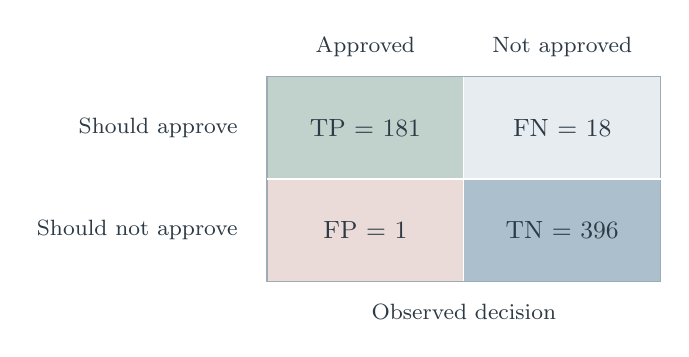
\begin{tikzpicture}[font=\small, text=evalInk, x=2.5cm, y=1.30cm]
\fill[evalTeal!54!white] (0,0) rectangle (1,-1);
\fill[evalBlue!20!white] (1,0) rectangle (2,-1);
\fill[evalRose!40!white] (0,-1) rectangle (1,-2);
\fill[evalBlue!67!white] (1,-1) rectangle (2,-2);
\draw[evalSlate] (0,0) rectangle (2,-2);
\draw[white] (1,0)--(1,-2) (0,-1)--(2,-1);
\node[evalInk] at (.5,-.5) {TP = 181};
\node at (1.5,-.5) {FN = 18};
\node at (.5,-1.5) {FP = 1};
\node[evalInk] at (1.5,-1.5) {TN = 396};
\node[anchor=east,font=\footnotesize] at (-0.1,-.5) {Should approve};
\node[anchor=east,font=\footnotesize] at (-0.1,-1.5) {Should not approve};
\node[font=\footnotesize,anchor=south] at (.5,0.10) {Approved};
\node[font=\footnotesize,anchor=south] at (1.5,0.10) {Not approved};
\node[font=\footnotesize] at (1,-2.3) {Observed decision};
\end{tikzpicture}
\caption{Binary approval confusion matrix for 596 completed decisions}
\label{fig:results_binary_matrix}
\end{figure}



\begin{table}[H]
\centering\small
\caption{Binary approval metrics for 596 completed decisions.}
\label{tab:results_binary_metrics}
\begin{tabular}{p{0.36\linewidth}p{0.29\linewidth}r}
\hline
\textbf{Measure} & \textbf{Calculation} & \textbf{Result} \\
\hline
Precision & $TP/(TP+FP)=181/182$ & 99.45\% \\
Recall & $TP/(TP+FN)=181/199$ & 90.95\% \\
Specificity & $TN/(TN+FP)=396/397$ & 99.75\% \\
False-positive rate & $FP/(FP+TN)=1/397$ & 0.25\% \\
False-negative rate & $FN/(FN+TP)=18/199$ & 9.05\% \\
F1 score & $2TP/(2TP+FP+FN)=362/381$ & 95.01\% \\
Binary accuracy & $(TP+TN)/596=577/596$ & 96.81\% \\
\hline
\end{tabular}
\end{table}

\subsection{Category Findings and Interpretation Errors}
\label{sec:results_errors_pairs}

\paragraph{Invalid relationships between known entities.}
All 100 requests in this category received the expected rejection,
without operational errors or false approvals. In 32 requests both assets
appeared in admitted Uniswap pools, but no admissible pool connected the
requested pair. The remaining 68 involved at least one known asset outside
the locally admitted Uniswap pool-asset set. These cases therefore also test
prototype admission policy, not exclusively missing relationships between
two admitted swap assets.

\paragraph{Unknown or unsupported entities and operations.}
This category produced 99 exact matches out of 100 requests. All 60 requests
specifying unsupported protocols, networks or actions were identified as
\texttt{UNSUPPORTED}. Of 38 requests using assets absent from the admitted
Aave reserves, 37 were rejected and one ended in a quota error. Two
native-asset boundary requests were rejected as expected. No false
approval was recorded. Absence from the local snapshot does not imply
that an asset is nonexistent or unsafe. Across the balanced study, 71 requests did not meet the joint-reference
criterion: 66 had a different final disposition and five had the expected
clarification status but mismatched fields. Figure~\ref{fig:results_errors}
shows the primary diagnoses obtained from retrospective inspection of the
recorded responses and validation results. The diagnoses were assigned retrospectively from stored responses and validation
records; they were not confirmed through a new execution after code changes.

\begin{figure}[H]
\centering
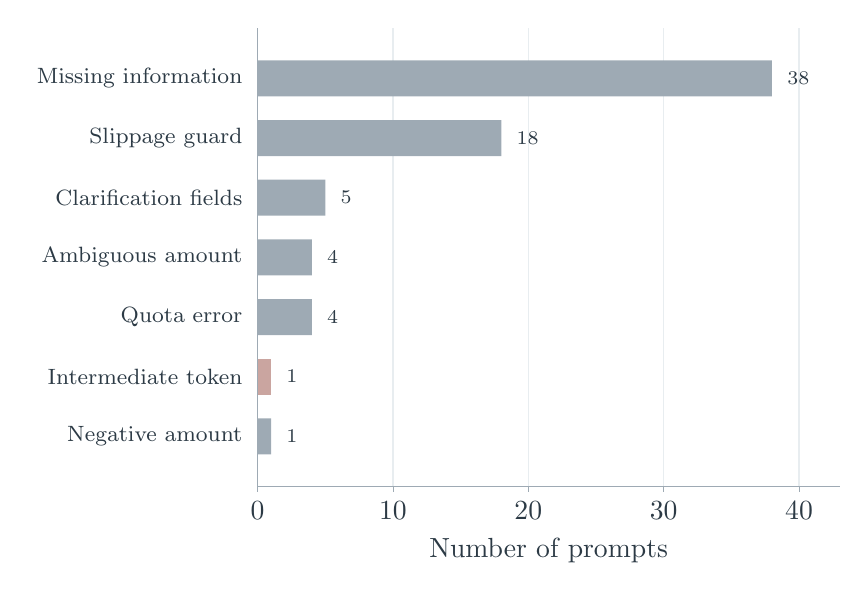
\begin{tikzpicture}
\begin{axis}[
    evaluationAxis,
    xbar,
    width=0.74\linewidth,
    height=7.4cm,
    xmin=0, xmax=43,
    xtick={0,10,20,30,40},
    xlabel={Number of prompts},
    xmajorgrids,
    grid style={evalGrid,line width=0.45pt},
    axis x line*=bottom,
    axis y line*=left,
    ytick style={draw=none},
    tick align=outside,
    major tick length=2pt,
    symbolic y coords={
        Negative amount,
        Intermediate token,
        Quota error,
        Ambiguous amount,
        Clarification fields,
        Slippage guard,
        Missing information
    },
    ytick={
        Negative amount,
        Intermediate token,
        Quota error,
        Ambiguous amount,
        Clarification fields,
        Slippage guard,
        Missing information
    },
    yticklabel style={font=\footnotesize,text=evalInk},
    enlarge y limits=0.14,
    enlarge x limits=false,
    bar width=13pt,
    bar shift=0pt,
    nodes near coords,
    point meta=x,
    every node near coord/.append style={
        font=\scriptsize,
        text=evalInk,
        anchor=west,
        xshift=2pt
    },
    clip=false,
]
\addplot[fill=evalSlate,draw=none] coordinates {
    (38,Missing information)
    (18,Slippage guard)
    (5,Clarification fields)
    (4,Ambiguous amount)
    (4,Quota error)
    (1,Negative amount)
};
\addplot[fill=evalRose,draw=none] coordinates {
    (1,Intermediate token)
};
\end{axis}
\end{tikzpicture}
\caption{Primary diagnoses for the 71 joint-reference mismatches. The highlighted intermediate-token case was the only false approval.}
\label{fig:results_errors}
\end{figure}

The 18 false negatives for supported Uniswap swaps all occurred in the
alternative wording. The model extracted the numerical slippage correctly,
but the deterministic text guard did not recognize expressions such as
``slippage must not exceed''. These requests were therefore marked
\texttt{UNSUPPORTED} before graph verification. In 38 incomplete requests, the model reported missing information as
an unsupported constraint, which took precedence over clarification.
Four further requests represented ambiguous amounts as prose and were
rejected. Five clarification responses omitted fields explicitly supplied
by the user.

One request received approval despite a draft reference requiring
non-approval. Its instruction was:
\begin{quote}
\emph{``On Ethereum Sepolia, use Uniswap V3 to swap an input of
23.8125 USDC for WETH; route through USDT as an intermediate token.''}
\end{quote}
The single false approval arose when the intent-generation model omitted
an intermediate-token requirement and produced a direct-swap intent.
The graph verifier approved this reduced intent because its specified
direct path was admitted by the verification graph. The error therefore
occurred during interpretation of the original request, rather than in
the graph verifier's assessment of the resulting direct-swap intent.
The draft reference remains subject to researcher review, and no
transaction was submitted.

To examine sensitivity to wording, each of the 300 evaluation scenarios
was expressed in two forms: a primary formulation and an alternative
formulation. The final status returned for each wording was compared
with the corresponding draft-reference status. As shown in
Figure~\ref{fig:results_pairs}, both wordings matched the reference in
250 pairs; only the primary wording matched in 24 pairs, only the
alternative wording in 10, and neither wording in 16. The two observed
statuses were identical in 263 pairs (87.67\%), although identical
outputs do not necessarily agree with the reference. Under the stricter
joint criterion, requiring agreement on both final status and selected
structured-intent fields, both wordings matched in 246 pairs (82.00\%).
These results describe paired formulations of the same scenarios, not
independent observations.

\begin{figure}[H]
\centering
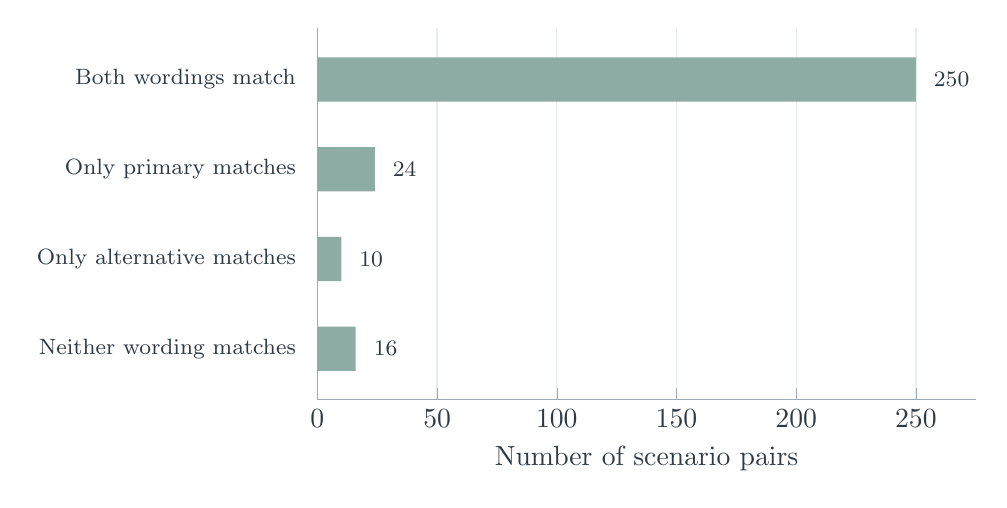
\begin{tikzpicture}
\begin{axis}[
    evaluationAxis,
    xbar,
    width=0.82\linewidth,
    height=6.3cm,
    xmin=0, xmax=275,
    xtick={0,50,100,150,200,250},
    xlabel={Number of scenario pairs},
    xmajorgrids,
    grid style={evalGrid,line width=0.45pt},
    symbolic y coords={
        Neither wording matches,
        Only alternative matches,
        Only primary matches,
        Both wordings match
    },
    ytick={
        Neither wording matches,
        Only alternative matches,
        Only primary matches,
        Both wordings match
    },
    yticklabel style={font=\footnotesize,text=evalInk},
    ytick style={draw=none},
    bar width=16pt,
    bar shift=0pt,
    enlarge y limits=0.19,
    enlarge x limits=false,
    axis x line*=bottom,
    axis y line*=left,
    nodes near coords,
    point meta=x,
    every node near coord/.append style={
        font=\footnotesize,
        text=evalInk,
        anchor=west,
        xshift=3pt
    },
    clip=false
]
\addplot[fill=evalTeal,draw=none] coordinates {
    (16,Neither wording matches)
    (10,Only alternative matches)
    (24,Only primary matches)
    (250,Both wordings match)
};
\end{axis}
\end{tikzpicture}
\caption{Draft-reference final-status agreement across 300 pairs of
alternative formulations. Each pair represents two wordings of the
same evaluation scenario.}
\label{fig:results_pairs}
\end{figure}

\subsection{Independent Graph Verification and Performance}
\label{sec:results_graph_latency}

Experiment B submitted eligible reference intents directly to the graph
verifier, regardless of language-model extraction. All 340 calls matched
the draft decisions and selected execution evidence derived from the
admitted graph snapshot. They covered 170 paired scenarios but only
112 distinct graph inputs. This establishes snapshot conformance, not
independent verification of every underlying protocol fact or a complete
audit trail for rejected relationships. The verifier returned a decision within two seconds for 338 of 340 calls
(99.41\%). Among the first occurrences of the 112 distinct inputs,
110 met the threshold (98.21\%). Both populations meet the measured
R6 target of at least 95\% within two seconds, although they are not
independent workloads. The two slow calls lasted 12,327.911 ms and
2,549.117 ms; neither was excluded from the analysis. 

\begin{table}[htbp]
\centering\small
\caption{Direct reference-intent graph-verification latency.}
\label{tab:results_graph_latency}
\begin{tabular}{p{0.32\linewidth}rrrr}
\hline
\textbf{Population} & \textbf{Within 2 s} & \textbf{Median (ms)} &
\textbf{P95 (ms)} & \textbf{Max. (ms)} \\
\hline
All 340 calls & 338 (99.41\%) & 16.815 & 29.827 & 12,327.911 \\
First of 112 distinct inputs & 110 (98.21\%) & 16.684 & 58.905 & 12,327.911 \\
\hline
\end{tabular}
\end{table}

\begin{figure}[H]
\centering
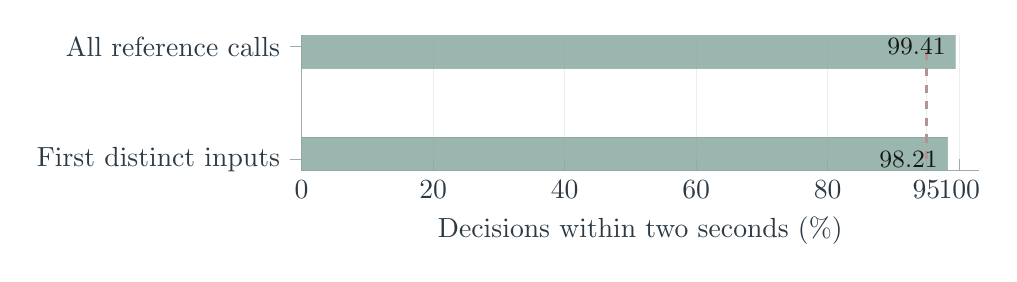
\begin{tikzpicture}
\begin{axis}[
    evaluationAxis,
  xbar,width=.84\linewidth,height=3.3cm,xmin=0,xmax=103,
  symbolic y coords={First distinct inputs,All reference calls},ytick=data,
  xlabel={Decisions within two seconds (\%)},
  xtick={0,20,40,60,80,95,100},
  xmajorgrids,grid style={evalGrid},
  bar width=16pt,
  nodes near coords,every node near coord/.append style={font=\small,anchor=east},
  axis x line*=bottom,axis y line*=left,
]
\addplot[fill=evalTeal,draw=evalTeal!75!evalInk,fill opacity=0.88,draw opacity=0.35] coordinates {
  (98.21,First distinct inputs) (99.41,All reference calls)};
\draw[evalRose!85!evalInk,dashed,thick] (axis cs:95,First distinct inputs) -- (axis cs:95,All reference calls);
\end{axis}
\end{tikzpicture}
\caption{Proportion of graph-verification calls completed within the two-second
R6 threshold (dashed line at 95\%).}
\label{fig:results_latency}
\end{figure}

Figure~\ref{fig:results_latency} shows that all first and slow calls are retained and both plotted populations draw from the same run and are not independent.
The recorded timings include Cypher and database processing but exclude
model extraction, wallet preparation and blockchain execution. The measured
proportions apply to this test environment and do not establish a general
latency guarantee. A separate post-change timing regression from 24 October 2026 included
the additional diagnostic processing. Of 340 reference-intent calls,
339 (99.71\%) completed within two seconds; for first occurrences of
112 distinct inputs, 111 (99.11\%) met the threshold. Both proportions
satisfy R6 in this recorded workload. These measurements are separate
from the earlier results reported above and are not combined with them.


\subsection{Controlled Verification and Execution Tests}
\label{sec:results_controlled}

In the separate relationship-mutation experiment, both the full graph
verifier and an entity-existence baseline approved all 12 valid controls.
After removal of one required relationship, the graph verifier rejected
all 60 mutations, whereas the baseline approved all 60. The mutations
derive from 12 fixtures, so the comparison demonstrates the contribution
of connected relationship checks within those fixtures rather than a
population-wide detection rate. Figure~\ref{fig:results_mutation_baseline} shows that the results are grouped by the 12 underlying graph
fixtures; this is a controlled comparison, not a population estimate.

\begin{figure}[htbp]
\centering
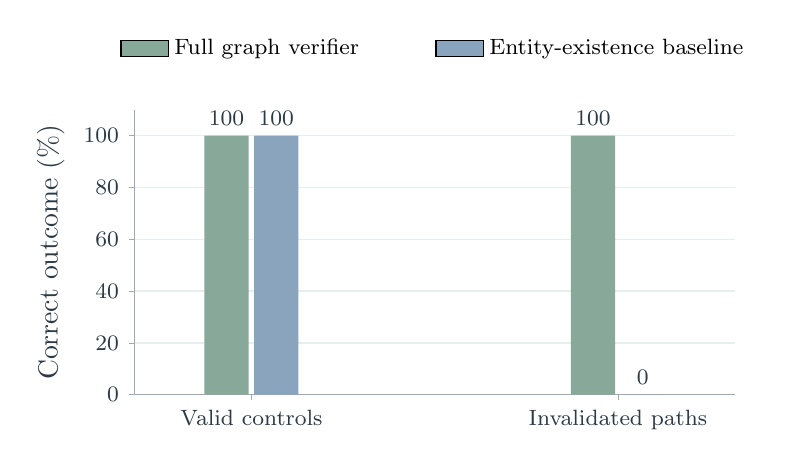
\begin{tikzpicture}
\definecolor{evalGreenSoft}{HTML}{88A89A}
\definecolor{evalBlueSoft}{HTML}{89A4BC}
\begin{axis}[
    evaluationAxis,
    ybar,
    width=0.76\linewidth,
    height=5.2cm,
    ymin=0,
    ymax=110,
    ytick={0,20,40,60,80,100},
    ylabel={Correct outcome (\%)},
    symbolic x coords={Valid controls,Invalidated paths},
    xtick=data,
    xticklabel style={font=\footnotesize, text=evalInk},
    yticklabel style={font=\footnotesize, text=evalInk},
    axis x line*=bottom,
    axis y line*=left,
    tick align=outside,
    major tick length=2pt,
    ymajorgrids,
    grid style={evalGrid,line width=0.45pt},
    bar width=16pt,
    enlarge x limits=0.32,
    nodes near coords,
    point meta=y,
    every node near coord/.append style={
        font=\footnotesize,
        text=evalInk
    },
    legend style={
        at={(0.5,1.14)},
        anchor=south,
        legend columns=2,
        draw=none,
        font=\footnotesize,
        /tikz/every even column/.append style={column sep=0.9cm}
    },
    clip=false
]
\addplot[
    fill=evalGreenSoft,
    draw=none,
    bar shift=-9pt,
    forget plot
] coordinates {
    (Valid controls,100)
    (Invalidated paths,100)
};
\addplot[
    fill=evalBlueSoft,
    draw=none,
    bar shift=9pt,
    forget plot
] coordinates {
    (Valid controls,100)
    (Invalidated paths,0)
};
\addlegendimage{area legend,fill=evalGreenSoft,draw=none}
\addlegendentry{Full graph verifier}
\addlegendimage{area legend,fill=evalBlueSoft,draw=none}
\addlegendentry{Entity-existence baseline}
\end{axis}
\end{tikzpicture}
\caption{Correct approvals of the 12 valid controls and correct non-approvals
of the 60 altered paths.}
\label{fig:results_mutation_baseline}
\end{figure}

The knowledge-maintenance experiment produced 36 recorded results
across 12 controlled conditions, with three repetitions per condition.
All matched the predefined expectations. Stale or incomplete knowledge
prevented approval, while deactivated relationships were rejected when
coverage was declared complete. Simulated database failures were handled
as operational conditions. A strict traceability audit of the 72 relationship-test results found
explicit decisions in every case but no stable rule identifiers. Only
the 12 valid controls contained the specific expected relationship evidence;
none of the 60 mutation rejections identified the deleted edge and its
expected and observed values. Correct decisions therefore did not provide
complete explanatory traceability.

\noindent\textbf{Post-change traceability evaluation.}
The verification-result mechanism was subsequently extended with
rule-based diagnostics. A paired regression recorded on 24 October 2026
reused the 12 valid controls and 60 single-relationship mutations. All
72 verification decisions remained unchanged. For the 60 mutations,
the revised verifier identified the deleted relationship, including
its type and endpoints, and reported the applicable expected and
observed conditions in every case. For example, one Uniswap mutation
identified a missing \texttt{EXPOSES\_FUNCTION} relationship between the
router contract and \texttt{exactInputSingle}. Thus all four R5
criteria were demonstrated for this mutation subset. The result does not extend to every verification output. All 12 approved
controls retained the expected execution evidence but lacked an explicit
reason or verification-rule identifier, so R5 criterion C2 was not met
for these cases. Across the separate reference-intent and boundary
workloads, 13 results retained generic \texttt{not\_localized} diagnostics.
The 36 recorded knowledge-lifecycle calls preserved the distinction
between rejected relationships and insufficient evidence without
inventing specific missing relationships. Across 462 paired cases,
no decision changed after the diagnostic extension. A subsequent review
on 27 October reran 46 offline tests successfully and re-audited the
saved records, but could not perform new live graph tests because Neo4j
was unavailable.


Finally, 28 implemented wallet-policy and handover tests matched their
expected results. There are some limitations in which should be focused such as,
connected-wallet and backend-signer binding, cumulative ERC-20 spending
budgets, and persistent receipt reconciliation. Several responses were
simulated, and these tests did not establish live transaction success.

\noindent\textbf{Restricted wallet-authorization evaluation.}
A subsequent implementation extension was assessed through
213 passing Python tests and 74 passing JavaScript tests.
The Python results included existing regression tests and
new authorization-related tests. The JavaScript evaluation
included contract-level tests using the actual Kernel and
ERC-4337 EntryPoint implementations. All five supported operation patterns were executed successfully
in the local contract environment. Negative tests confirmed
rejection of modified destinations, functions, amounts,
recipients, approval spenders, transaction batches, and
authorization conditions. The validator also enforced
permission validity and single-use restrictions. These
results demonstrate independent wallet-level enforcement
for the tested operations, rather than backend-only rejection. The revised authorization mechanism was not installed on
public Ethereum Sepolia. Public-bundler compatibility and
successful testnet settlement therefore remain unverified.

% 5.4 discussion


\section{Discussion}
\label{sec:evaluation_discussion}

The results indicate that action-specific graph verification can establish
whether an interpreted DeFi operation follows the relationships admitted to
the knowledge graph. However, the correctness of the complete pipeline also
depends on preserving the original request. The difference between exact-status
and binary approval agreement is particularly relevant here: treating all
non-approval outcomes as equivalent conceals whether a request was correctly
rejected, classified as unsupported, or identified as requiring clarification.

The natural-language experiments exposed weaknesses primarily in constraint
handling and incomplete requests. In 18 supported Uniswap cases, the model
extracted the slippage value correctly, but deterministic validation did not
recognize the wording and prevented further verification. Other incomplete
requests were classified as unsupported rather than requiring clarification.
More importantly, a request to swap USDC for WETH through USDT as an
intermediate token was reduced to a direct swap. The graph verifier approved
the reduced operation, demonstrating that a valid graph path cannot establish
that an omitted user condition has been respected. No transaction was submitted.

The graph-specific experiments provide stronger evidence for the relationship
checks themselves. Reference-intent verification matched the admitted graph
snapshot, independently of language-model extraction. In the controlled
mutation experiment, the full verifier rejected all 60 altered paths while
the entity-existence baseline approved them. This shows why checking the
existence of contracts, functions, and assets separately is insufficient
when their required connections are invalid. It does not establish that
Neo4j is the only data model capable of performing these checks.

The knowledge-maintenance experiments further demonstrated the distinction
between an unsupported relationship and insufficient evidence. Stale or
incomplete knowledge prevented approval, whereas a deactivated relationship
could be rejected under declared complete coverage. A failed update did not
necessarily invalidate a previously admitted snapshot that remained current.
Verification latency met the two-second target of R6 for the measured graph
workloads, although individual slow calls remained. These results support
feasibility within the tested environment rather than a general performance
guarantee.

The experiments also revealed several limitations of the implemented prototype:

\begin{itemize}
    \item \textbf{Intent preservation.} The system can lose an explicit condition
    before graph verification. Different formulations can also produce
    different validation outcomes, particularly for slippage and ambiguity.

    \item \textbf{Verification knowledge.} Decisions depend on the correctness,
    freshness, and coverage of the admitted snapshot. The local Uniswap
    asset-admission restriction is a prototype policy, not an official
    dependency on Aave.

    \item \textbf{Execution control.}
The implementation demonstrates restricted wallet-level
authorization in a local contract environment. However, public
Sepolia installation, bundler acceptance, authenticated binding
to the connected browser-wallet owner, and cumulative spending
budgets across separate approvals remain unverified or
incomplete. The validator also depends on a trusted verification
authority and has not undergone an independent security audit.

    
\item \textbf{Traceability.} The revised verifier identified all 60
controlled missing relationships, but approved controls did not provide
an explicit reason or verification-rule identifier and some broader
requests retained generic diagnostics. Complete traceability for every
outcome was therefore not demonstrated.

\end{itemize}

An earlier exploratory study conducted on 19 and 20 October 2026
included 400 prompts. Of these, 344 (86.00\%) matched the drafted
final-status references and 336 (84.00\%) met the recorded joint
criterion. The exploratory study informed subsequent development,
but its dataset and procedure differed from the balanced evaluation.
The difference in aggregate agreement therefore cannot establish
a causal improvement. Both studies relied on assistant-drafted
references without documented independent item-level review.

% 5.5
\section{Requirements Evaluation}
\label{sec:requirements_evaluation}

The prototype is assessed against requirements R1 to R6 using the criteria defined
in Section~\ref{sec:requirements_analysis}. The qualitative assessment scale
for R1 to R5 and the separate latency scale for R6 are retained from
Tables~\ref{tab:general_assessment_scale} and~\ref{tab:r6_scale} in Chapter~\ref{chap:stateoftheart}. The ratings reflect the experimental evidence
and the mandatory criteria of each requirement, rather than the number of
technologies combined in the prototype.

\begingroup
\providecommand{\evThree}{\ensuremath{\bigstar\,\bigstar\,\bigstar}}
\providecommand{\evTwo}{\ensuremath{\bigstar\,\bigstar\,\circ}}
\providecommand{\evOne}{\ensuremath{\bigstar\,\circ\,\circ}}
\providecommand{\evZero}{\ensuremath{\circ\,\circ\,\circ}}

\noindent\textbf{R1: Complete and Unambiguous Structured Intent.}
The prototype produces structured intents and validates action-specific fields.
However, the language experiments found that incomplete instructions were
sometimes classified as unsupported and that an intermediate-token condition
could be omitted. The criteria concerning representation and mandatory fields
are supported, while consistent handling of ambiguity is not. R1 receives
\evTwo. Agreement with the assistant-drafted references does not establish
independently validated intent accuracy.

\medskip\noindent\textbf{R2: Intent-to-Execution Relationship Validation.}
Graph verification checks deployment, action, contract, function and resource
relationships before execution. All 340 direct reference-intent calls matched
the selected evidence and decisions of the admitted snapshot. In the controlled
comparison, the full verifier rejected all 60 relationship mutations that
an entity-existence baseline approved. These results support all four criteria
within the evaluated scope, giving R2 \evThree. They do not independently
establish the correctness of every protocol fact stored in the graph.

\medskip\noindent\textbf{R3: Authoritative and Maintainable Verification Knowledge.}
Protocol-specific acquisition records identifiable sources and deployment
context. The graph retains provenance, validity and freshness information,
and supports updating or invalidating relationships. Controlled lifecycle
experiments confirmed the expected handling of stale and incomplete knowledge,
relationship deactivation and simulated availability failures. The implemented
capabilities support R3 \evThree\ within the prototype scope. Continuous
correctness of all external protocol information was not established.



\noindent\textbf{R4: Pre-Execution Enforcement and Controlled Execution.}
The prototype implements a verification boundary that prevents
non-approved operations from proceeding through the intended
execution workflow. Approved operations are retained server-side,
checked for expiry and reuse, and reverified before execution.
The original demonstration used ERC-4337 through ZeroDev Kernel,
but did not enforce comprehensive wallet-level restrictions. A subsequent implementation extension introduced a restricted
smart-account validator that binds authorization to the complete
approved transaction batch. The mechanism uses separate owner,
verification-authority, and execution-signer roles. It restricts
the executable operation through exact calldata binding,
account and network restrictions, limited validity, and
single-use authorization.

Controlled tests using the actual Kernel and ERC-4337 EntryPoint
contracts confirmed successful execution of the five supported
operation patterns and rejection of unauthorized modifications.
All four R4 criteria, including the mandatory enforcement
criteria C2 and C3, were therefore supported within the locally
evaluated scope. Consequently, the revised implementation
receives \evThree{}. The restricted validator was not installed on public Ethereum
Sepolia, and public-bundler acceptance and production-level
security were not established.




\medskip\noindent\textbf{R5: Traceable Verification Result.}
The initial traceability audit found that rejected relationship
mutations did not identify the failed connection. After the diagnostic
extension, the verifier correctly localized all 60 controlled missing
relationships, including their endpoints and applicable expected and
observed conditions. Explicit decisions were preserved, and these
mutation cases satisfied all four R5 criteria. However, the 12 valid
controls lacked a reason or verification-rule identifier (C2), and
13 additional graph results retained generic, non-localized diagnostics.
The revised implementation therefore provides substantial but
incomplete traceability within the evaluated scope. R5 receives \evTwo;
the available evidence does not establish full coverage across all
verification outcomes.



\medskip\noindent\textbf{R6: Bounded Verification Time.}
Of the 340 direct reference-intent calls, 338 completed within two seconds
(99.41\%). The first occurrences of 112 distinct graph inputs achieved
110 timely results (98.21\%). Both recorded populations exceed the 95\%
threshold defined for R6 and support \evThree\ for the tested environment.
The calculation retains the slow calls and excludes language-model generation
and wallet processing. It is not a worst-case performance guarantee.

Table~\ref{tab:evaluation_approach_comparison} compares the prototype with the
five approach groups assessed using the assessment criteria from Chapter~\ref{chap:stateoftheart}. Their original ratings are
unchanged. \textit{N/E} indicates insufficient comparable evidence, rather
than a negative assessment.

\begin{table}[htbp]
    \centering
    \small
    \setlength{\tabcolsep}{3pt}
    \caption{Requirement coverage of existing approach groups and the
    implemented prototype}
    \label{tab:evaluation_approach_comparison}
    \begin{tabular}{>{\raggedright\arraybackslash}p{5.8cm}cccccc}
        \hline
        \textbf{Approach group} & \textbf{R1} & \textbf{R2} &
        \textbf{R3} & \textbf{R4} & \textbf{R5} & \textbf{R6} \\
        \hline
        Execution-Layer Security and Policy Enforcement
          & \evZero & \evOne & \evOne & \evThree & \evTwo & N/E \\
        AI-Agent Blockchain Execution
          & \evTwo & \evTwo & \evOne & \evOne & \evTwo & N/E \\
        Knowledge Retrieval and Grounding
          & \evZero & \evOne & \evOne & \evZero & \evZero & N/E \\
        Graph-Based Relationship Analysis
          & \evZero & \evOne & \evOne & \evZero & \evOne & N/E \\
        Smart Contract Security Analysis
          & \evZero & \evZero & \evOne & \evZero & \evOne & N/E \\
        \hline
\textbf{Implemented prototype}
  & \evTwo & \evThree & \evThree & \evThree & \evTwo & \evThree \\
        \hline
    \end{tabular}
\end{table}

The prototype combines intent interpretation, maintained verification
knowledge, and pre-execution relationship checks that existing approach
groups usually address separately. Its strongest demonstrated contribution
is the validation of connected execution relationships. The revised
traceability mechanism provides more specific diagnostic evidence, supporting
the R5 assessment, while the restricted wallet-authorization extension strengthens R4
by enforcing approved execution conditions independently of
backend checks in the locally evaluated contract environment.
This complements the graph-based verification mechanism,
although deployment and validation through a public Sepolia
bundler remain outside the demonstrated scope. The comparison applies the common requirement criteria rather
than a direct experimental benchmark against the reviewed systems.


\endgroup

% 5.6

\section{Threats to Validity}
\label{sec:evaluation_threats}

The experimental findings are subject to several validity threats. These
concern the reliability and generalizability of the evaluation rather than
the prototype's functional limitations.

\medskip\noindent\textbf{Internal validity.}
The natural-language requests and reference outcomes were drafted with
assistant support and were not independently adjudicated by human reviewers.
Shared assumptions or errors may therefore affect the reported agreement.
Moreover, findings from the exploratory 400-prompt study informed the later
600-prompt dataset, which was not an untouched independent test set. The two
studies also used different scenario distributions, so differences between
their aggregate results do not establish a causal improvement. Four provider
quota errors were retained in the final study, but one execution period cannot
establish the long-term consistency of the external language-model service.

\medskip\noindent\textbf{Construct validity.}
Exact-status agreement measures consistency with drafted references, not
complete preservation of every original user condition. Binary approval
metrics also conceal differences between rejection, unsupported scope, and
clarification. The joint agreement measure checks selected fields only for
specified approved and clarification references. Similarly, independent graph
results establish agreement with the admitted snapshot rather than independent
on-chain correctness of every protocol fact. The entity-existence baseline
represents a deliberately limited alternative, while the mutation experiments
cover missing relationships rather than all possible execution-data errors.
The original wallet-handover evaluation relied partly on
simulated outcomes, while the subsequent authorization extension
was tested against actual smart-account contracts in a local EVM.
These local tests establish enforcement of the selected permission
conditions but not public-bundler compatibility, testnet
installation, production security, or successful DeFi settlement.

\medskip\noindent\textbf{External validity.}
The experiments cover selected Uniswap V3 and Aave V3 operations and assets
on Ethereum Sepolia. Synthetic, partly template-based requests may not reflect
the linguistic diversity, adversarial inputs, or changing conditions of
operational DeFi agents. The relationship mutations and injected knowledge
failures are controlled scenarios rather than representative samples of real
contract migrations, unreliable sources, or infrastructure outages. The
findings therefore cannot be generalized directly to other protocols,
networks, or production environments.

\medskip\noindent\textbf{Statistical conclusion validity.}
The 600 prompts comprise two formulations of 300 scenarios, while 340
reference-intent graph calls include only 112 distinct graph inputs. Repeated
and related observations cannot be treated as independent real-world samples.
Agreement rates and latency percentiles are therefore reported descriptively,
without independent-sample confidence intervals or significance claims.
The two slow graph calls and the observed false approval remain relevant;
their rarity in these experiments does not establish deployment probabilities.

Separating evaluation stages, retaining errors, and reporting paired and
distinct-input results reduce some of these risks. Stronger conclusions would
require independently reviewed references, more diverse deployments, and
repeated operational measurements. Any later implementation changes must be
supported by separate regression evidence.

% 5.7

\section{Summary}
\label{sec:evaluation_summary}

This chapter evaluated the prototype's intent processing, graph-based
relationship verification, knowledge maintenance, execution controls,
traceability, and verification time against the requirements defined in
Chapter~\ref{chap:stateoftheart}.

The balanced 600-prompt experiment achieved 89.00\% exact-status agreement
with the drafted references. Although binary approval classification was
more accurate, the results revealed difficulties with ambiguous requests
and preservation of user-specified constraints. In particular, an omitted
intermediate-token condition led to approval of a simplified swap. This
demonstrates that correct relationship verification cannot compensate for
an incorrectly interpreted intent. The independent graph experiment produced the expected snapshot-based
decisions in all 340 calls. Furthermore, the relationship verifier rejected
all 60 controlled relationship mutations that the entity-existence baseline
approved. Knowledge-maintenance tests demonstrated appropriate non-approval
behaviour under stale or incomplete evidence, while 99.41\% of reference-intent
verification calls completed within two seconds. These findings support the
effectiveness and feasibility of the proposed mechanism within the tested
scope. 

The requirements evaluation found strong coverage of relationship validation,
verification knowledge, and measured verification time. 
The initial traceability limitations were addressed through additional
deterministic diagnostics. A separate regression correctly localized
all 60 controlled missing relationships without changing the
verification decisions. However, incomplete reason information for
approved controls and generic diagnostics in some other cases prevent
a claim of complete traceability. The revised verifier also met the
specified latency target in the recorded post-change workload. Targeted
regression tests supported the revised R5 assessment. Intent preservation remains a limitation of the complete
pipeline. The subsequent restricted wallet-authorization
extension strengthens execution enforcement and satisfies R4
within the locally evaluated scope, while public testnet
deployment and production-level assurance remain unverified.

Overall, the evaluation supports the central contribution of this thesis:
explicit verification of action-specific DeFi execution relationships provides
an additional safeguard between AI-generated intent and blockchain execution.
Its effectiveness nevertheless depends on faithful intent interpretation,
reliable verification knowledge, and appropriate execution restrictions.
The findings remain limited to the evaluated protocols, network, and
experimental conditions.

